

\tikzset{every picture/.style={line width=0.75pt}} %set default line width to 0.75pt        

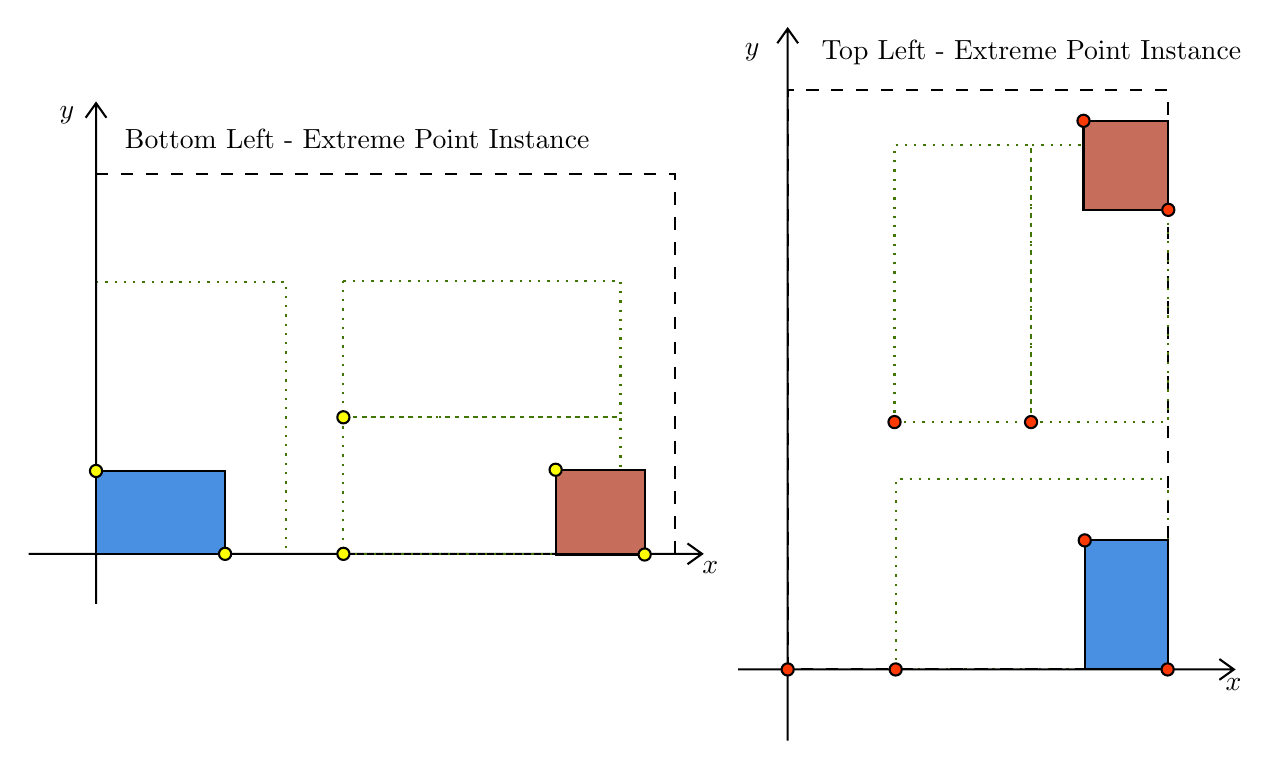
\begin{tikzpicture}[x=0.75pt,y=0.75pt,yscale=-1,xscale=1]
%uncomment if require: \path (0,380); %set diagram left start at 0, and has height of 380

%Shape: Rectangle [id:dp676391404304541] 
\draw  [color={rgb, 255:red, 65; green, 117; blue, 5 }  ,draw opacity=1 ][dash pattern={on 0.84pt off 2.51pt}] (65.44,151.69) -- (157,151.69) -- (157,282.71) -- (65.44,282.71) -- cycle ;
%Shape: Rectangle [id:dp26001178837889305] 
\draw  [color={rgb, 255:red, 65; green, 117; blue, 5 }  ,draw opacity=1 ][dash pattern={on 0.84pt off 2.51pt}] (450.7,338.41) -- (450.7,246.85) -- (581.72,246.85) -- (581.72,338.41) -- cycle ;
%Shape: Rectangle [id:dp532870934725963] 
\draw  [dash pattern={on 4.5pt off 4.5pt}] (65.44,99.66) -- (344.58,99.66) -- (344.58,282.71) -- (65.44,282.71) -- cycle ;
%Shape: Axis 2D [id:dp545947560183275] 
\draw  (33,282.71) -- (357.39,282.71)(65.44,65.6) -- (65.44,306.84) (350.39,277.71) -- (357.39,282.71) -- (350.39,287.71) (60.44,72.6) -- (65.44,65.6) -- (70.44,72.6)  ;
%Shape: Rectangle [id:dp13640021794487145] 
\draw  [fill={rgb, 255:red, 74; green, 144; blue, 226 }  ,fill opacity=1 ] (65.44,242.78) -- (127.61,242.78) -- (127.61,282.71) -- (65.44,282.71) -- cycle ;
%Shape: Ellipse [id:dp4997787088203596] 
\draw  [fill={rgb, 255:red, 252; green, 255; blue, 4 }  ,fill opacity=1 ] (62.5,242.78) .. controls (62.5,241.16) and (63.82,239.84) .. (65.44,239.84) .. controls (67.06,239.84) and (68.38,241.16) .. (68.38,242.78) .. controls (68.38,244.4) and (67.06,245.72) .. (65.44,245.72) .. controls (63.82,245.72) and (62.5,244.4) .. (62.5,242.78) -- cycle ;
%Shape: Ellipse [id:dp9368091558454169] 
\draw  [fill={rgb, 255:red, 252; green, 255; blue, 4 }  ,fill opacity=1 ] (124.67,282.71) .. controls (124.67,281.09) and (125.99,279.77) .. (127.61,279.77) .. controls (129.24,279.77) and (130.55,281.09) .. (130.55,282.71) .. controls (130.55,284.34) and (129.24,285.65) .. (127.61,285.65) .. controls (125.99,285.65) and (124.67,284.34) .. (124.67,282.71) -- cycle ;
%Shape: Rectangle [id:dp10130767347226488] 
\draw  [color={rgb, 255:red, 65; green, 117; blue, 5 }  ,draw opacity=1 ][dash pattern={on 0.84pt off 2.51pt}] (184.62,216.92) -- (318.13,216.92) -- (318.13,282.71) -- (184.62,282.71) -- cycle ;
%Shape: Rectangle [id:dp8859988076373574] 
\draw  [color={rgb, 255:red, 65; green, 117; blue, 5 }  ,draw opacity=1 ][dash pattern={on 0.84pt off 2.51pt}] (184.62,151.14) -- (318.13,151.14) -- (318.13,216.92) -- (184.62,216.92) -- cycle ;
%Shape: Rectangle [id:dp5346376956315015] 
\draw  [fill={rgb, 255:red, 198; green, 110; blue, 91 }  ,fill opacity=1 ] (286.87,242.19) -- (329.77,242.19) -- (329.77,283.04) -- (286.87,283.04) -- cycle ;
%Shape: Ellipse [id:dp5380867242688693] 
\draw  [fill={rgb, 255:red, 252; green, 255; blue, 4 }  ,fill opacity=1 ] (181.68,282.71) .. controls (181.68,281.09) and (182.99,279.77) .. (184.62,279.77) .. controls (186.24,279.77) and (187.55,281.09) .. (187.55,282.71) .. controls (187.55,284.34) and (186.24,285.65) .. (184.62,285.65) .. controls (182.99,285.65) and (181.68,284.34) .. (181.68,282.71) -- cycle ;
%Shape: Circle [id:dp32824759445274065] 
\draw  [fill={rgb, 255:red, 252; green, 255; blue, 4 }  ,fill opacity=1 ] (181.68,216.92) .. controls (181.68,215.3) and (182.99,213.99) .. (184.62,213.99) .. controls (186.24,213.99) and (187.55,215.3) .. (187.55,216.92) .. controls (187.55,218.55) and (186.24,219.86) .. (184.62,219.86) .. controls (182.99,219.86) and (181.68,218.55) .. (181.68,216.92) -- cycle ;
%Shape: Rectangle [id:dp013806976369067359] 
\draw  [dash pattern={on 4.5pt off 4.5pt}] (398.67,338.41) -- (398.67,59.27) -- (581.72,59.27) -- (581.72,338.41) -- cycle ;
%Shape: Axis 2D [id:dp26544149420697416] 
\draw  (374.78,338.41) -- (613.65,338.41)(398.67,29.71) -- (398.67,372.71) (606.65,333.41) -- (613.65,338.41) -- (606.65,343.41) (393.67,36.71) -- (398.67,29.71) -- (403.67,36.71)  ;
%Shape: Rectangle [id:dp4452985784509189] 
\draw  [fill={rgb, 255:red, 74; green, 144; blue, 226 }  ,fill opacity=1 ] (541.79,338.41) -- (541.79,276.23) -- (581.72,276.23) -- (581.72,338.41) -- cycle ;
%Shape: Rectangle [id:dp24524128214266327] 
\draw  [color={rgb, 255:red, 65; green, 117; blue, 5 }  ,draw opacity=1 ][dash pattern={on 0.84pt off 2.51pt}] (515.93,219.23) -- (515.93,85.71) -- (581.72,85.71) -- (581.72,219.23) -- cycle ;
%Shape: Rectangle [id:dp5234703657507643] 
\draw  [color={rgb, 255:red, 65; green, 117; blue, 5 }  ,draw opacity=1 ][dash pattern={on 0.84pt off 2.51pt}] (450.14,219.23) -- (450.14,85.71) -- (515.93,85.71) -- (515.93,219.23) -- cycle ;
%Shape: Rectangle [id:dp9419058705222738] 
\draw  [fill={rgb, 255:red, 198; green, 110; blue, 91 }  ,fill opacity=1 ] (541.2,116.98) -- (541.2,74.08) -- (582.04,74.08) -- (582.04,116.98) -- cycle ;
%Shape: Ellipse [id:dp3331578572136539] 
\draw  [fill={rgb, 255:red, 255; green, 57; blue, 4 }  ,fill opacity=1 ] (450.14,222.17) .. controls (448.52,222.17) and (447.21,220.85) .. (447.21,219.23) .. controls (447.21,217.61) and (448.52,216.29) .. (450.14,216.29) .. controls (451.77,216.29) and (453.08,217.61) .. (453.08,219.23) .. controls (453.08,220.85) and (451.77,222.17) .. (450.14,222.17) -- cycle ;
%Shape: Ellipse [id:dp23570925769851603] 
\draw  [fill={rgb, 255:red, 255; green, 57; blue, 4 }  ,fill opacity=1 ] (515.93,222.17) .. controls (514.31,222.17) and (512.99,220.85) .. (512.99,219.23) .. controls (512.99,217.61) and (514.31,216.29) .. (515.93,216.29) .. controls (517.56,216.29) and (518.87,217.61) .. (518.87,219.23) .. controls (518.87,220.85) and (517.56,222.17) .. (515.93,222.17) -- cycle ;
%Shape: Ellipse [id:dp5636473664839672] 
\draw  [fill={rgb, 255:red, 255; green, 57; blue, 4 }  ,fill opacity=1 ] (450.7,341.35) .. controls (449.08,341.35) and (447.76,340.03) .. (447.76,338.41) .. controls (447.76,336.78) and (449.08,335.47) .. (450.7,335.47) .. controls (452.33,335.47) and (453.64,336.78) .. (453.64,338.41) .. controls (453.64,340.03) and (452.33,341.35) .. (450.7,341.35) -- cycle ;
%Shape: Ellipse [id:dp310194773919646] 
\draw  [fill={rgb, 255:red, 255; green, 57; blue, 4 }  ,fill opacity=1 ] (581.72,341.35) .. controls (580.1,341.35) and (578.78,340.03) .. (578.78,338.41) .. controls (578.78,336.78) and (580.1,335.47) .. (581.72,335.47) .. controls (583.34,335.47) and (584.66,336.78) .. (584.66,338.41) .. controls (584.66,340.03) and (583.34,341.35) .. (581.72,341.35) -- cycle ;
%Shape: Ellipse [id:dp4413085834987862] 
\draw  [fill={rgb, 255:red, 255; green, 57; blue, 4 }  ,fill opacity=1 ] (541.79,279.17) .. controls (540.17,279.17) and (538.85,277.86) .. (538.85,276.23) .. controls (538.85,274.61) and (540.17,273.29) .. (541.79,273.29) .. controls (543.41,273.29) and (544.73,274.61) .. (544.73,276.23) .. controls (544.73,277.86) and (543.41,279.17) .. (541.79,279.17) -- cycle ;
%Shape: Ellipse [id:dp9184751088799129] 
\draw  [fill={rgb, 255:red, 252; green, 255; blue, 4 }  ,fill opacity=1 ] (326.83,283.04) .. controls (326.83,281.41) and (328.14,280.1) .. (329.77,280.1) .. controls (331.39,280.1) and (332.71,281.41) .. (332.71,283.04) .. controls (332.71,284.66) and (331.39,285.97) .. (329.77,285.97) .. controls (328.14,285.97) and (326.83,284.66) .. (326.83,283.04) -- cycle ;
%Shape: Ellipse [id:dp412533006945518] 
\draw  [fill={rgb, 255:red, 252; green, 255; blue, 4 }  ,fill opacity=1 ] (283.93,242.19) .. controls (283.93,240.57) and (285.25,239.26) .. (286.87,239.26) .. controls (288.49,239.26) and (289.81,240.57) .. (289.81,242.19) .. controls (289.81,243.82) and (288.49,245.13) .. (286.87,245.13) .. controls (285.25,245.13) and (283.93,243.82) .. (283.93,242.19) -- cycle ;
%Shape: Ellipse [id:dp37052430797411673] 
\draw  [fill={rgb, 255:red, 255; green, 57; blue, 4 }  ,fill opacity=1 ] (582.04,119.92) .. controls (580.42,119.92) and (579.11,118.6) .. (579.11,116.98) .. controls (579.11,115.35) and (580.42,114.04) .. (582.04,114.04) .. controls (583.67,114.04) and (584.98,115.35) .. (584.98,116.98) .. controls (584.98,118.6) and (583.67,119.92) .. (582.04,119.92) -- cycle ;
%Shape: Ellipse [id:dp8764279608687702] 
\draw  [fill={rgb, 255:red, 255; green, 57; blue, 4 }  ,fill opacity=1 ] (541.2,77.02) .. controls (539.58,77.02) and (538.26,75.7) .. (538.26,74.08) .. controls (538.26,72.46) and (539.58,71.14) .. (541.2,71.14) .. controls (542.82,71.14) and (544.14,72.46) .. (544.14,74.08) .. controls (544.14,75.7) and (542.82,77.02) .. (541.2,77.02) -- cycle ;
%Shape: Ellipse [id:dp6792036584804988] 
\draw  [fill={rgb, 255:red, 255; green, 57; blue, 4 }  ,fill opacity=1 ] (398.67,341.35) .. controls (397.04,341.35) and (395.73,340.03) .. (395.73,338.41) .. controls (395.73,336.78) and (397.04,335.47) .. (398.67,335.47) .. controls (400.29,335.47) and (401.6,336.78) .. (401.6,338.41) .. controls (401.6,340.03) and (400.29,341.35) .. (398.67,341.35) -- cycle ;

% Text Node
\draw (46.39,65.64) node [anchor=north west][inner sep=0.75pt]    {$y$};
% Text Node
\draw (356.09,284.84) node [anchor=north west][inner sep=0.75pt]    {$x$};
% Text Node
\draw (77.86,76.79) node [anchor=north west][inner sep=0.75pt]   [align=left] {Bottom Left - Extreme Point Instance};
% Text Node
\draw (376.52,35.3) node [anchor=north west][inner sep=0.75pt]    {$y$};
% Text Node
\draw (608.21,341.49) node [anchor=north west][inner sep=0.75pt]    {$x$};
% Text Node
\draw (413.49,33.94) node [anchor=north west][inner sep=0.75pt]   [align=left] {Top Left - Extreme Point Instance};


\end{tikzpicture}
